\subsection{Soil Desiccation}

\subsectioncover

\begin{frame}{}
\vspace{-1.5em}
\begin{columns}
    \begin{column}{0.3\textwidth}
        \vspace{-1em}
        \begin{figure}[htb!]
            \centering
            \begin{subfigure}[b]{\textwidth}
                \centering
                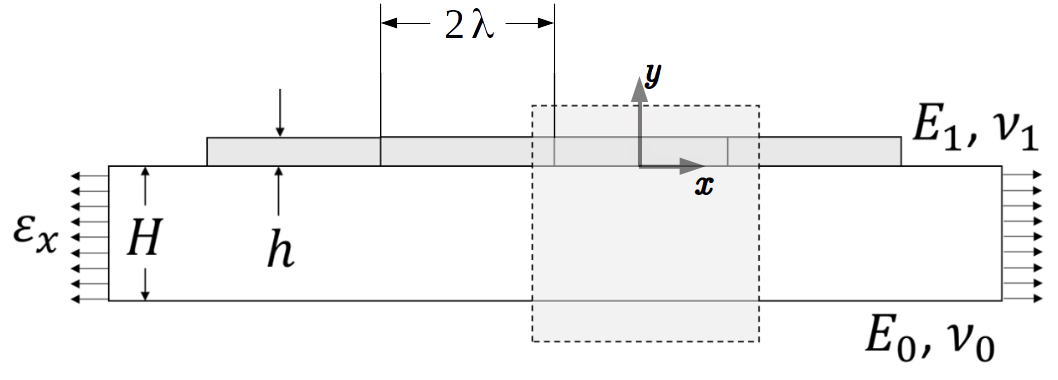
\includegraphics[width=0.8\textwidth]{past/figures/1D_schematic.png}
                \caption{}
            \end{subfigure}

            \begin{subfigure}[b]{\textwidth}
                \centering
                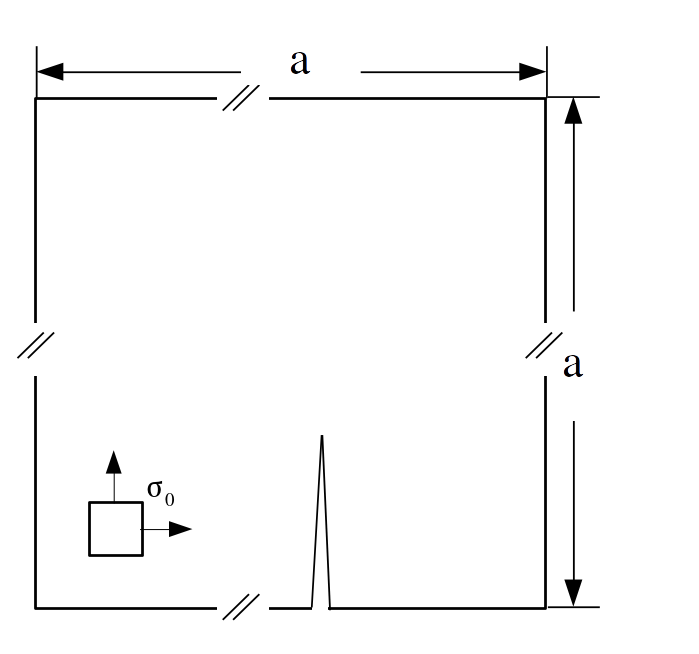
\includegraphics[width=0.5\textwidth]{past/figures/2D_schematic.png}
                \caption{}
            \end{subfigure}

            \begin{subfigure}[b]{\textwidth}
                \centering
                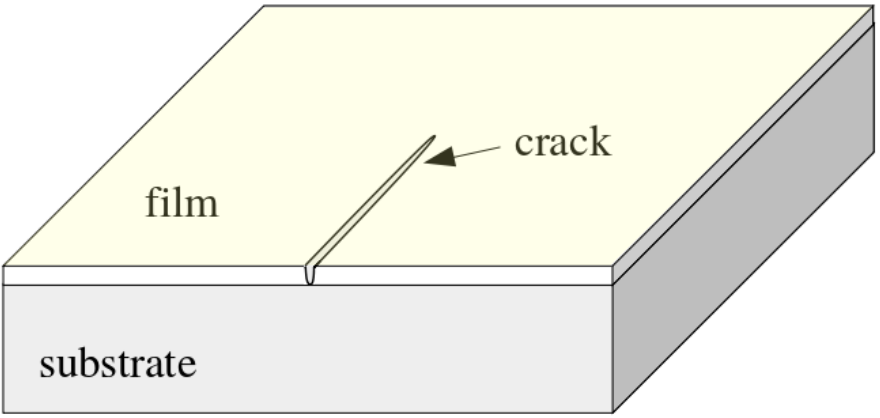
\includegraphics[width=0.6\textwidth]{past/figures/3D_schematic.png}
                \caption{}
            \end{subfigure}
        \end{figure}
        \vspace{-1em}
        \begin{exampleblock}{}
          See \texttt{mud.pdf} for details.
        \end{exampleblock}
    \end{column}
    \begin{column}{0.7\textwidth}
        \begin{itemize}
            \item Only ``channeling'' cracks in the thin film are considered.
            \item Small deformation is assumed for $\pi_\elastic$, and $\strain = (\grad \bs{u} + \grad^T \bs{u})/2$.
            \item \textcolor<5>{dukeroyal}{A frictionless contact split of the elastic energy is applied at the vicinity of the crack set.}
            \item Thermal effects are neglected. Dehydration is modeled as pre-stress in $\pi_\inelastic = \sigma_0 \tr(\strain)$.
            \item A cohesive-type fracture model is used for $\pi_\fracture$.
            \pause
            \item The model is verified with analytical solutions in a periodic quasi-1D context (Fig.~a).
            \pause
            \item Pervasive fracture is studied with a 2D simplification (Fig.~b).
            \item The energy $\pi_\interface$ accounts for mismatch between the film and the substrate.
            \item \textcolor<5>{dukeroyal}{Material property inhomogeneity in the macroscopic continuum model is taken into account by introducing two pointwise correlated random fields $\{\Gc(\bs{X}), \bs{X} \in \body\}$ and $\{\pi_c(\bs{X}), \bs{X} \in \body\}$.}
            \pause
            \item \textcolor<5>{dukeroyal}{The versatility offered by the probabilistic framework is highlighted by solving a 3D problem based on physical experiments.}
        \end{itemize}
    \end{column}
\end{columns}
\end{frame}

\begin{frame}{}
\contenttitle{The contact split}\\
The elastic energy takes into account the tension-compression asymmetry and the frictionless contact condition at the vicinity of the crack set:
\begin{subequations}
\begin{align}
    \pi_\elastic &= g_{qq}(d; p) \pi_\elastic^\activeenergy + \pi_\elastic^\inactiveenergy, \\
    \pi_\elastic^\activeenergy &=
    \begin{cases}
        \dfrac{1}{2} \lambda_s \macaulay{\tr(\strain)}_+^2 + \mu_s \strain^+ : \strain^+, \quad d \leqslant d_\critical, \\
        \dfrac{1}{2} ( \stress_n^+ + \stress_t ) : \strain, \quad d > d_\critical,
    \end{cases} \\
    \pi_\elastic^\inactiveenergy &=
    \begin{cases}
        \dfrac{1}{2} \lambda_s \macaulay{\tr(\strain)}_-^2 + \mu_s \strain^- : \strain^-, \quad d \leqslant d_\critical, \\
        \dfrac{1}{2} \stress_n^- : \strain, \quad d > d_\critical,
    \end{cases}
\end{align}
\end{subequations}
\end{frame}

\begin{frame}{}
\begin{columns}
    \begin{column}{0.7\textwidth}
        \vspace{-2em}
        % !TEX root = ../../main.tex

\begin{figure}[htb!]
    \begin{subfigure}[b]{0.23\textwidth}
        \centering
        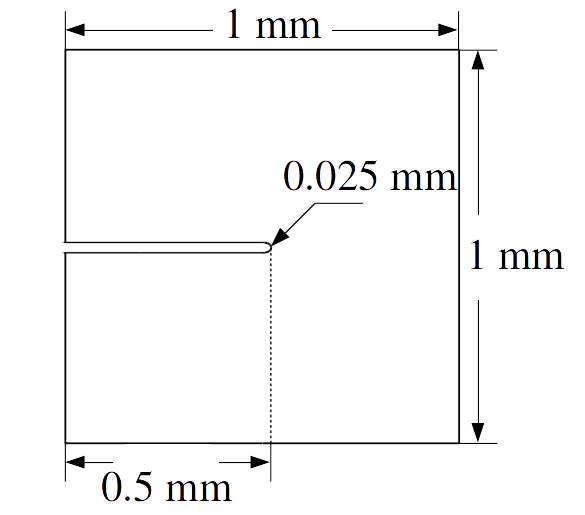
\includegraphics[width=\textwidth,scale=0.5]{past/figures/notched_plate_dimensions.png}
    \end{subfigure}
    \begin{subfigure}[b]{0.21\textwidth}
        \centering
        
\includegraphics[width=\textwidth,scale=0.5]{past/figures/notched_plate_initial.png}
    \end{subfigure}
    \begin{subfigure}[b]{0.21\textwidth}
        \centering
        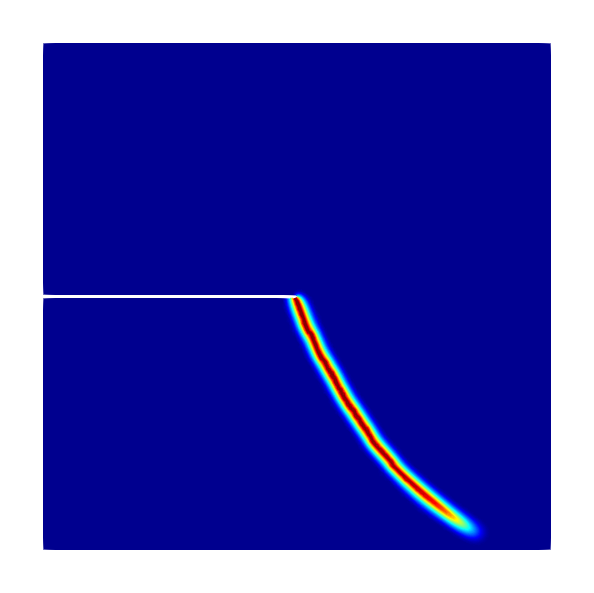
\includegraphics[width=\textwidth,scale=0.5]{past/figures/mode2_notched_plate_spectral_intermediate.png}
    \end{subfigure}
    \begin{subfigure}[b]{0.21\textwidth}
        \centering
        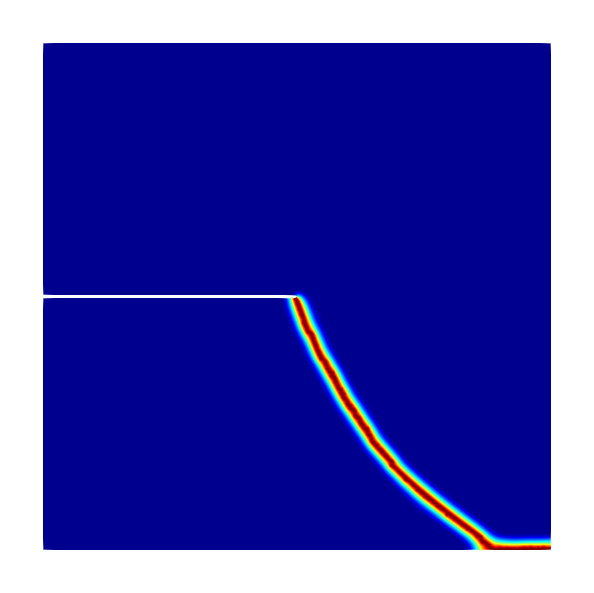
\includegraphics[width=\textwidth,scale=0.5]{past/figures/mode2_notched_plate_spectral_final.png}
    \end{subfigure}
    \begin{subfigure}[b]{0.06\textwidth}
        \centering
        \caption*{d}
        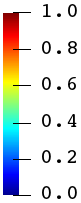
\includegraphics[width=\textwidth]{colorbar/jet_vertical.png}
    \end{subfigure}

    \hspace{0.015\textwidth}
    \begin{subfigure}[b]{0.21\textwidth}
        \centering
        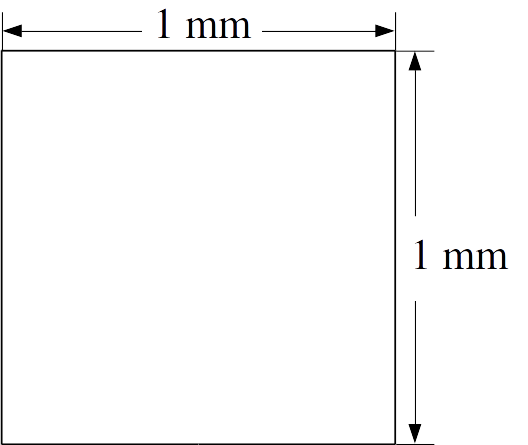
\includegraphics[width=\textwidth,scale=0.5]{past/figures/intact_plate_dimensions.png}
        \vspace{-0.03\textwidth}
    \end{subfigure}
    \begin{subfigure}[b]{0.21\textwidth}
        \centering
        
\includegraphics[width=\textwidth,scale=0.5]{past/figures/intact_plate_initial.png}
    \end{subfigure}
    \begin{subfigure}[b]{0.21\textwidth}
        \centering
        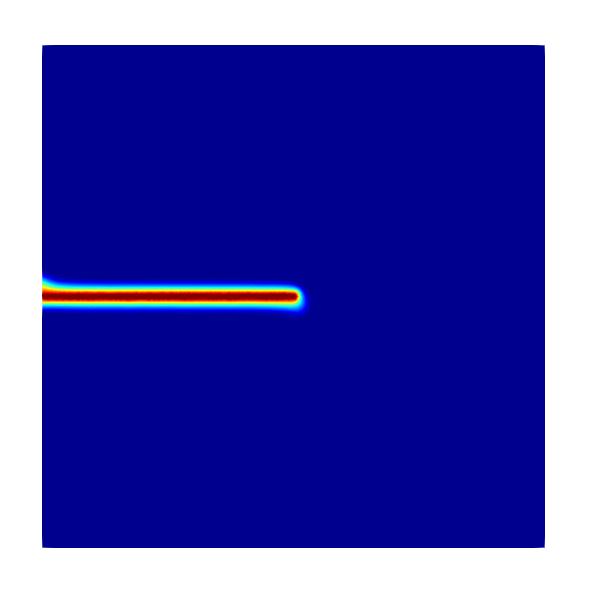
\includegraphics[width=\textwidth,scale=0.5]{past/figures/mode2_intact_plate_spectral_intermediate.png}
    \end{subfigure}
    \begin{subfigure}[b]{0.21\textwidth}
        \centering
        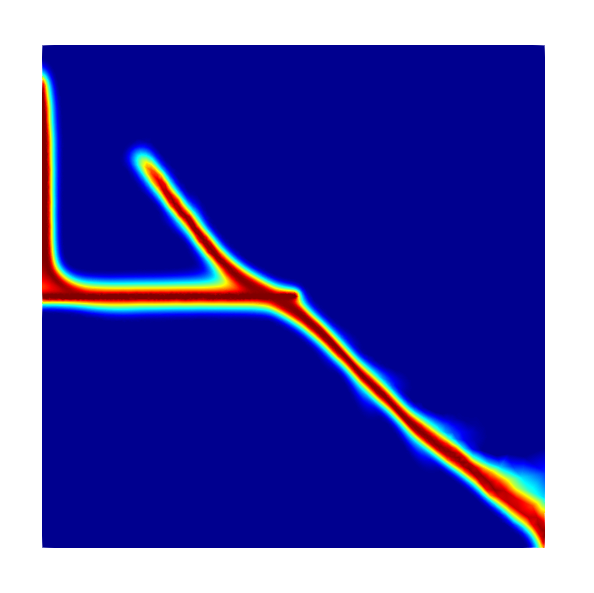
\includegraphics[width=\textwidth,scale=0.5]{past/figures/mode2_intact_plate_spectral_final.png}
    \end{subfigure}
    \begin{subfigure}[b]{0.06\textwidth}
        \centering
        \caption*{d}
        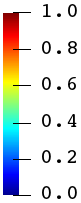
\includegraphics[width=\textwidth]{colorbar/jet_vertical.png}
    \end{subfigure}

    \hspace{0.015\textwidth}
    \begin{subfigure}[b]{0.21\textwidth}
        \centering
        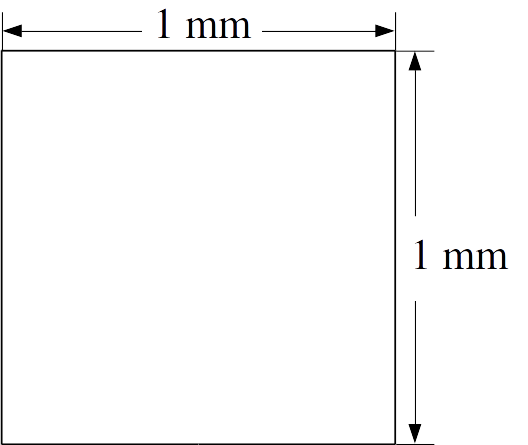
\includegraphics[width=\textwidth,scale=0.5]{past/figures/intact_plate_dimensions.png}
        \vspace{-0.03\textwidth}
    \end{subfigure}
    \begin{subfigure}[b]{0.21\textwidth}
        \centering
        
\includegraphics[width=\textwidth,scale=0.5]{past/figures/intact_plate_initial.png}
    \end{subfigure}
    \begin{subfigure}[b]{0.21\textwidth}
        \centering
        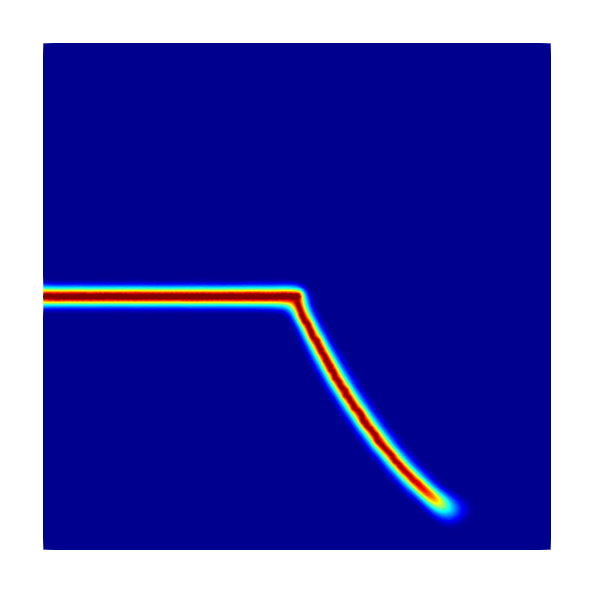
\includegraphics[width=\textwidth,scale=0.5]{past/figures/mode2_intact_plate_odd_intermediate.png}
    \end{subfigure}
    \begin{subfigure}[b]{0.21\textwidth}
        \centering
        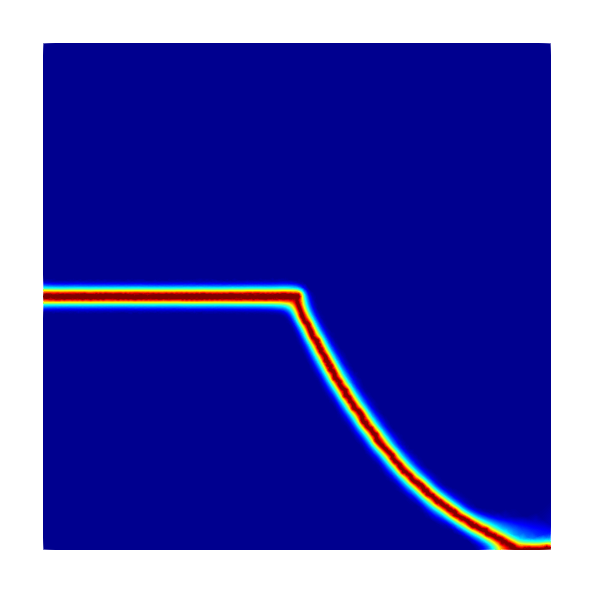
\includegraphics[width=\textwidth,scale=0.5]{past/figures/mode2_intact_plate_odd_final.png}
    \end{subfigure}
    \begin{subfigure}[b]{0.06\textwidth}
        \centering
        \caption*{d}
        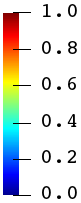
\includegraphics[width=\textwidth]{colorbar/jet_vertical.png}
    \end{subfigure}
\end{figure}

    \end{column}
    \begin{column}{0.3\textwidth}
        The crack paths obtained using \\
        (1st row) the spectral decomposition on a geometrically notched plate, \\
        (2nd row) the spectral decomposition with an initial damage field, \\
        (3rd row) the contact split with an initial damage field. \\
        \bigskip
        Snapshots of crack paths are shown at \\
        (2nd column) $u_x = \SI{0}{\milli\meter}$, \\
        (3rd column) $u_x = \SI{0.0109}{\milli\meter}$, \\
        (4th column) $u_x = \SI{0.02}{\milli\meter}$.
    \end{column}
\end{columns}
\end{frame}

\begin{frame}{}
\contenttitle{Material inhomogeneity} \\
The covariance function $\tau \mapsto \cor(\tau)$ for a $[0, L]^n$ $p$-periodic domain is given by
\begin{align}
    \cor(\tau) =
    \begin{bmatrix}
        \cor_1(\tau) & \rho \cor_1(\tau) \\
        \rho \cor_1(\tau) & \rho^2 \cor_1(\tau) + (1-\rho^2) \cor_2(\tau)
    \end{bmatrix}, \quad \forall \tau \in [0,p], \rho \in [-1, 1],
\end{align}
where the univariate covariance function $\cor$ is assumed to take the generic form
\begin{align}
    \cor_\phi(\tau; L) & = \exp\left( -c \phi(\tau; L)\right )~, \quad \forall \tau \in [0,p]~.
\end{align} \\
$\phi$ is a $p$-periodic function taken as
\begin{align}
    \phi(\tau; L) =
    \begin{cases}
        \dfrac{|\sin\left( \pi\tau/p \right)|}{L}, \quad \text{(Periodic Exponential, PE),} \\
        \dfrac{\sin\left( \pi\tau/p \right)^2}{L^2}, \quad \text{(Periodic Squared-Exponential, PSE)}.
    \end{cases}
\end{align}
\end{frame}

\begin{frame}{}
\begin{columns}
    \begin{column}{0.7\textwidth}
        \contenttitle{Sensitivity to the correlation length $L$} \\
        % !TEX root = ../../../main.tex

\begin{figure}[!htb]
    \centering
    \begin{subfigure}[b]{0.15\textwidth}
        \caption*{$\Gc^*$}
        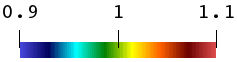
\includegraphics[width=\textwidth]{colorbar/rainbow_horizontal.png}
    \end{subfigure}
    \begin{subfigure}[b]{0.15\textwidth}
        \caption*{$\pi_c^*$}
        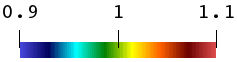
\includegraphics[width=\textwidth]{colorbar/rainbow_horizontal.png}
    \end{subfigure}
    \begin{subfigure}[b]{0.15\textwidth}
        \caption*{$d$}
        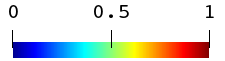
\includegraphics[width=\textwidth]{colorbar/jet_horizontal.png}
    \end{subfigure}
    \begin{subfigure}[b]{0.15\textwidth}
        \caption*{$\Gc^*$}
        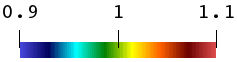
\includegraphics[width=\textwidth]{colorbar/rainbow_horizontal.png}
    \end{subfigure}
    \begin{subfigure}[b]{0.15\textwidth}
        \caption*{$\pi_c^*$}
        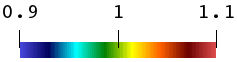
\includegraphics[width=\textwidth]{colorbar/rainbow_horizontal.png}
    \end{subfigure}
    \begin{subfigure}[b]{0.15\textwidth}
        \caption*{$d$}
        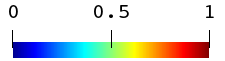
\includegraphics[width=\textwidth]{colorbar/jet_horizontal.png}
    \end{subfigure}

    \begin{subfigure}[b]{0.15\textwidth}
        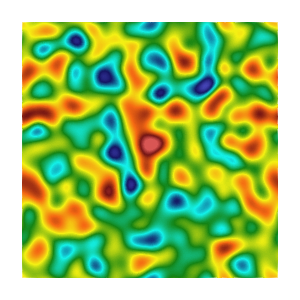
\includegraphics[width=\textwidth]{past/figures/Gc_sqexp_cartesian_5_5_rho_0_seed_a.png}
    \end{subfigure}
    \begin{subfigure}[b]{0.15\textwidth}
        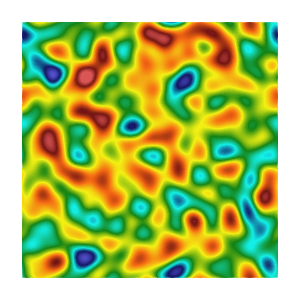
\includegraphics[width=\textwidth]{past/figures/psic_sqexp_cartesian_5_5_rho_0_seed_a.png}
    \end{subfigure}
    \begin{subfigure}[b]{0.15\textwidth}
        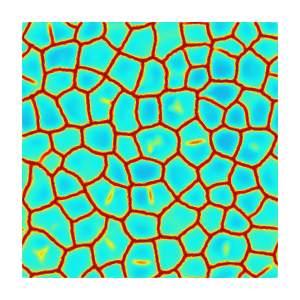
\includegraphics[width=\textwidth]{past/figures/d_sqexp_cartesian_5_5_rho_0_seed_a.png}
    \end{subfigure}
    \begin{subfigure}[b]{0.15\textwidth}
        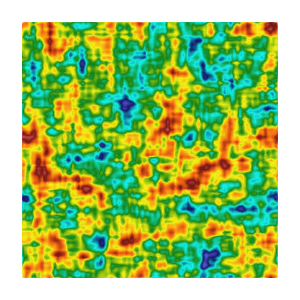
\includegraphics[width=\textwidth]{past/figures/Gc_exp_cartesian_5_5_rho_0_seed_b.png}
    \end{subfigure}
    \begin{subfigure}[b]{0.15\textwidth}
        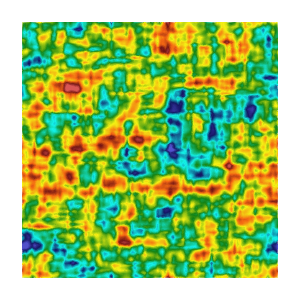
\includegraphics[width=\textwidth]{past/figures/psic_exp_cartesian_5_5_rho_0_seed_b.png}
    \end{subfigure}
    \begin{subfigure}[b]{0.15\textwidth}
        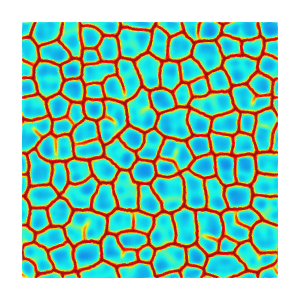
\includegraphics[width=\textwidth]{past/figures/d_exp_cartesian_5_5_rho_0_seed_b.png}
    \end{subfigure}

    \begin{subfigure}[b]{0.15\textwidth}
        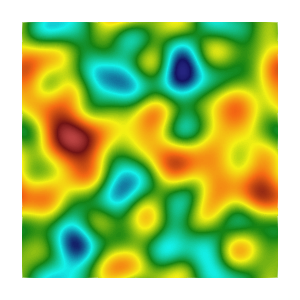
\includegraphics[width=\textwidth]{past/figures/Gc_sqexp_cartesian_10_10_rho_0_seed_a.png}
    \end{subfigure}
    \begin{subfigure}[b]{0.15\textwidth}
        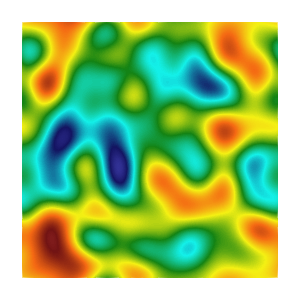
\includegraphics[width=\textwidth]{past/figures/psic_sqexp_cartesian_10_10_rho_0_seed_a.png}
    \end{subfigure}
    \begin{subfigure}[b]{0.15\textwidth}
        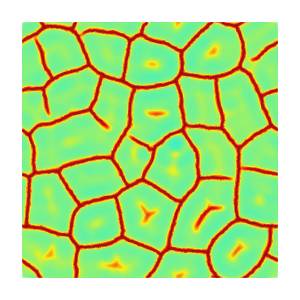
\includegraphics[width=\textwidth]{past/figures/d_sqexp_cartesian_10_10_rho_0_seed_a.png}
    \end{subfigure}
    \begin{subfigure}[b]{0.15\textwidth}
        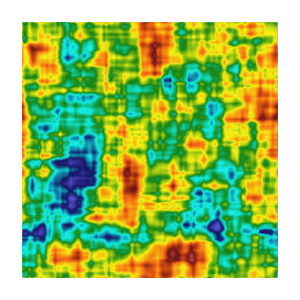
\includegraphics[width=\textwidth]{past/figures/Gc_exp_cartesian_10_10_rho_0_seed_b.png}
    \end{subfigure}
    \begin{subfigure}[b]{0.15\textwidth}
        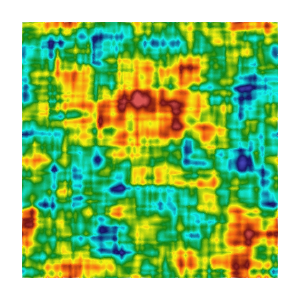
\includegraphics[width=\textwidth]{past/figures/psic_exp_cartesian_10_10_rho_0_seed_b.png}
    \end{subfigure}
    \begin{subfigure}[b]{0.15\textwidth}
        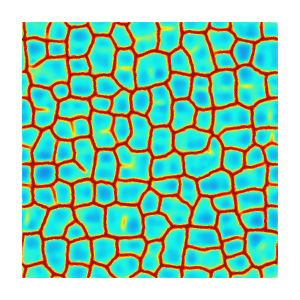
\includegraphics[width=\textwidth]{past/figures/d_exp_cartesian_10_10_rho_0_seed_b.png}
    \end{subfigure}

    \begin{subfigure}[b]{0.15\textwidth}
        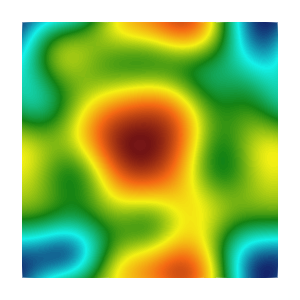
\includegraphics[width=\textwidth]{past/figures/Gc_sqexp_cartesian_20_20_rho_0_seed_a.png}
    \end{subfigure}
    \begin{subfigure}[b]{0.15\textwidth}
        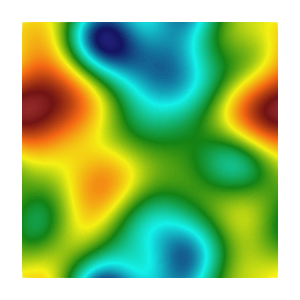
\includegraphics[width=\textwidth]{past/figures/psic_sqexp_cartesian_20_20_rho_0_seed_a.png}
    \end{subfigure}
    \begin{subfigure}[b]{0.15\textwidth}
        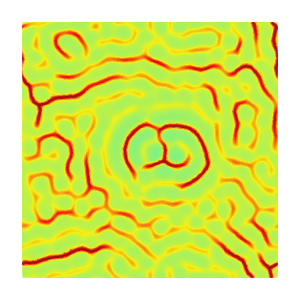
\includegraphics[width=\textwidth]{past/figures/d_sqexp_cartesian_20_20_rho_0_seed_a.png}
    \end{subfigure}
    \begin{subfigure}[b]{0.15\textwidth}
        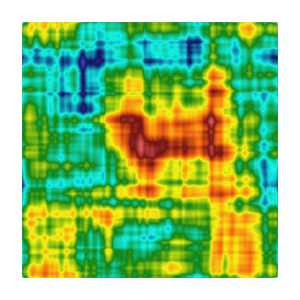
\includegraphics[width=\textwidth]{past/figures/Gc_exp_cartesian_20_20_rho_0_seed_b.png}
    \end{subfigure}
    \begin{subfigure}[b]{0.15\textwidth}
        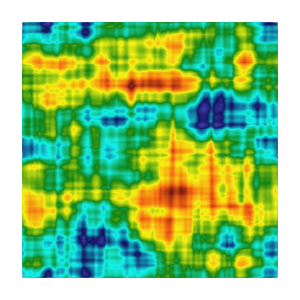
\includegraphics[width=\textwidth]{past/figures/psic_exp_cartesian_20_20_rho_0_seed_b.png}
    \end{subfigure}
    \begin{subfigure}[b]{0.15\textwidth}
        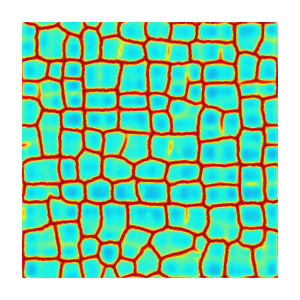
\includegraphics[width=\textwidth]{past/figures/d_exp_cartesian_20_20_rho_0_seed_b.png}
    \end{subfigure}
\end{figure}

    \end{column}
    \begin{column}{0.3\textwidth}
        \vspace{-2em}
        % !TEX root = ../../../main.tex

\begin{figure}[htb!]
    \centering
    \begin{subfigure}[b]{\textwidth}
        \centering
        \begin{tikzpicture}
            \begin{axis}[
                width=\textwidth,
                height=0.7\textwidth,
                ticks=none,
                ymode=log,
                log ticks with fixed point,
                ylabel=$\underline{l^*}$,xlabel=$\mathcal{D}^*$,
                % ymin=0,ymax=2.5
            ]
                \addplot [select coords between index={40}{220},color=black] table [x expr=\thisrowno{0},y expr=\thisrowno{1}]{past/data/dimensionless_curve_sqexp_cartesian_5_5.csv};
                \addplot [select coords between index={40}{220},color=red] table [x expr=\thisrowno{0},y expr=\thisrowno{1}]{past/data/dimensionless_curve_sqexp_cartesian_10_10.csv};
                \addplot [select coords between index={40}{220},color=blue] table [x expr=\thisrowno{0},y expr=\thisrowno{1}]{past/data/dimensionless_curve_sqexp_cartesian_20_20.csv};
            \end{axis}
        \end{tikzpicture}
    \end{subfigure}

    \begin{subfigure}[b]{\textwidth}
        \centering
        \begin{tikzpicture}
            \begin{axis}[
                width=\textwidth,
                height=0.7\textwidth,
                ticks=none,
                xlabel=$l^*$,ylabel=PDF,
                ymin=0,ymax=0.012,
                xmin=0,xmax=1000
            ]
                \addplot [color=black] table [x expr=\thisrowno{0},y expr=\thisrowno{1}]{past/data/distribution_sqexp_cartesian_5_5.csv};
                \addplot [color=red] table [x expr=\thisrowno{0},y expr=\thisrowno{1}]{past/data/distribution_sqexp_cartesian_10_10.csv};
                \addplot [color=blue] table [x expr=\thisrowno{0},y expr=\thisrowno{1}]{past/data/distribution_sqexp_cartesian_20_20.csv};
            \end{axis}
        \end{tikzpicture}
    \end{subfigure}

    \begin{subfigure}[b]{\textwidth}
        \centering
        \begin{tikzpicture}
            \begin{axis}[
                width=\textwidth,
                height=0.7\textwidth,
                ticks=none,
                ymode=log,
                log ticks with fixed point,
                ylabel=$\underline{l^*}$,xlabel=$\mathcal{D}^*$,
                % ymin=0,ymax=2.5
            ]
                \addplot [select coords between index={40}{220},color=black] table [x expr=\thisrowno{0},y expr=\thisrowno{1}]{past/data/dimensionless_curve_exp_cartesian_5_5.csv};
                \addplot [select coords between index={40}{220},color=red] table [x expr=\thisrowno{0},y expr=\thisrowno{1}]{past/data/dimensionless_curve_exp_cartesian_10_10.csv};
                \addplot [select coords between index={40}{220},color=blue] table [x expr=\thisrowno{0},y expr=\thisrowno{1}]{past/data/dimensionless_curve_exp_cartesian_20_20.csv};
            \end{axis}
        \end{tikzpicture}
    \end{subfigure}

    \begin{subfigure}[b]{\textwidth}
        \centering
        \begin{tikzpicture}
            \begin{axis}[
                width=\textwidth,
                height=0.7\textwidth,
                ticks=none,
                xlabel=$l^*$,ylabel=PDF,
                ymin=0,ymax=0.012,
                xmin=0,xmax=300
            ]
                \addplot [color=black] table [x expr=\thisrowno{0},y expr=\thisrowno{1}]{past/data/distribution_exp_cartesian_5_5.csv};
                \addplot [color=red] table [x expr=\thisrowno{0},y expr=\thisrowno{1}]{past/data/distribution_exp_cartesian_10_10.csv};
                \addplot [color=blue] table [x expr=\thisrowno{0},y expr=\thisrowno{1}]{past/data/distribution_exp_cartesian_20_20.csv};
            \end{axis}
        \end{tikzpicture}
    \end{subfigure}
\end{figure}

    \end{column}
\end{columns}
\end{frame}

\begin{frame}{}
\begin{columns}
    \begin{column}{0.7\textwidth}
        \contenttitle{Sensitivity to $\Gc$ and $\pi_c$} \\
        % !TEX root = ../../../main.tex

\begin{figure}[!htbp]
    \centering
    \begin{subfigure}[b]{0.07\textwidth}
        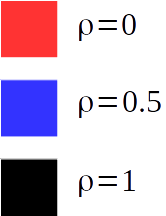
\includegraphics[width=\textwidth]{colorbar/rho.png}
        \vspace{0.2in}
    \end{subfigure}
    \begin{subfigure}[b]{0.35\textwidth}
        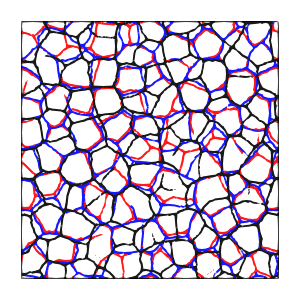
\includegraphics[width=0.6\textwidth]{past/figures/psic_constant.png}
    \end{subfigure}
    \begin{subfigure}[b]{0.07\textwidth}
        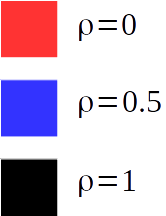
\includegraphics[width=\textwidth]{colorbar/rho.png}
        \vspace{0.2in}
    \end{subfigure}
    \begin{subfigure}[b]{0.35\textwidth}
        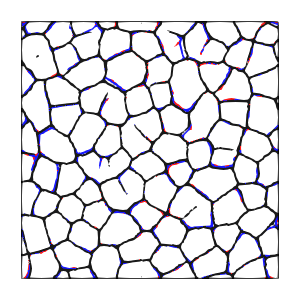
\includegraphics[width=0.6\textwidth]{past/figures/Gc_constant.png}
    \end{subfigure}
    
    \begin{subfigure}[b]{0.25\textwidth}
        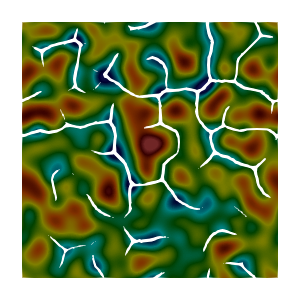
\includegraphics[width=0.7\textwidth]{past/figures/Gc_sqexp_cartesian_5_5_rho_0_seed_a_with_crack_140.png}
    \end{subfigure}
    \begin{subfigure}[b]{0.25\textwidth}
        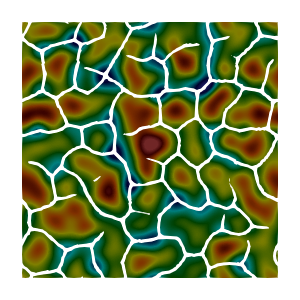
\includegraphics[width=0.7\textwidth]{past/figures/Gc_sqexp_cartesian_5_5_rho_0_seed_a_with_crack_160.png}
    \end{subfigure}
    \begin{subfigure}[b]{0.25\textwidth}
        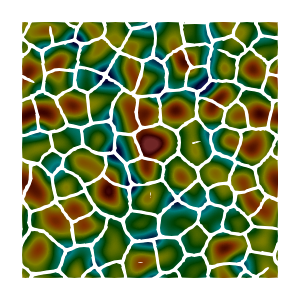
\includegraphics[width=0.7\textwidth]{past/figures/Gc_sqexp_cartesian_5_5_rho_0_seed_a_with_crack_220.png}
    \end{subfigure}
    \begin{subfigure}[b]{0.05\textwidth}
        \caption*{$\Gc^*$}
        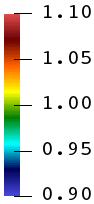
\includegraphics[width=\textwidth]{colorbar/rainbow_vertical.png}
    \end{subfigure}

    \begin{subfigure}[b]{0.25\textwidth}
        \includegraphics[width=0.7\textwidth]{past/figures/psic_sqexp_cartesian_5_5_rho_0_seed_a_with_crack_140.png}
    \end{subfigure}
    \begin{subfigure}[b]{0.25\textwidth}
        \includegraphics[width=0.7\textwidth]{past/figures/psic_sqexp_cartesian_5_5_rho_0_seed_a_with_crack_160.png}
    \end{subfigure}
    \begin{subfigure}[b]{0.25\textwidth}
        \includegraphics[width=0.7\textwidth]{past/figures/psic_sqexp_cartesian_5_5_rho_0_seed_a_with_crack_220.png}
    \end{subfigure}
    \begin{subfigure}[b]{0.05\textwidth}
        \caption*{$\pi_c^*$}
        \includegraphics[width=\textwidth]{colorbar/rainbow_vertical.png}
    \end{subfigure}
\end{figure}

    \end{column}
    \begin{column}{0.3\textwidth}
        \vspace{-2em}
        % !TEX root = ../../../main.tex

\begin{figure}[!htb]
    \centering
    \begin{subfigure}[b]{\textwidth}
        \centering
        \begin{tikzpicture}
            \begin{axis}[
                width=\textwidth,
                height=0.7\textwidth,
                ticks=none,
                ymode=log,
                log ticks with fixed point,
                ylabel=$\underline{l^*}$,xlabel=$\mathcal{D}^*$,
                % ymin=0,ymax=2.5
            ]
                % rho = 0
                \addplot [select coords between index={40}{220},color=red] table [x expr=\thisrowno{0},y expr=\thisrowno{1}]{past/data/dimensionless_curve_sqexp_rho_1.csv};
                % rho = 0.5
                \addplot [select coords between index={40}{220},color=blue] table [x expr=\thisrowno{0},y expr=\thisrowno{1}]{past/data/dimensionless_curve_sqexp_rho_2.csv};
                % rho = 1
                \addplot [select coords between index={40}{220},color=black] table [x expr=\thisrowno{0},y expr=\thisrowno{1}]{past/data/dimensionless_curve_sqexp_rho_3.csv};
            \end{axis}
        \end{tikzpicture}
    \end{subfigure}

    \begin{subfigure}[b]{\textwidth}
        \centering
        \begin{tikzpicture}
            \begin{axis}[
                width=\textwidth,
                height=0.7\textwidth,
                ticks=none,
                xlabel=$l^*$,ylabel=PDF,
                ymin=0,ymax=0.012,
                xmin=0,xmax=300
            ]
                \addplot [color=red] table [x expr=\thisrowno{0},y expr=\thisrowno{1}]{past/data/distribution_sqexp_rho_1.csv};
                \addplot [color=blue] table [x expr=\thisrowno{0},y expr=\thisrowno{1}]{past/data/distribution_sqexp_rho_2.csv};
                \addplot [color=black] table [x expr=\thisrowno{0},y expr=\thisrowno{1}]{past/data/distribution_sqexp_rho_3.csv};
            \end{axis}
        \end{tikzpicture}
    \end{subfigure}

    \begin{subfigure}[b]{\textwidth}
        \centering
        \begin{tikzpicture}
            \begin{axis}[
                width=\textwidth,
                height=0.7\textwidth,
                ticks=none,
                ymode=log,
                log ticks with fixed point,
                ylabel=$\underline{l^*}$,xlabel=$\mathcal{D}^*$,
                % ymin=0,ymax=2.5
            ]
                % rho = 0
                \addplot [select coords between index={40}{220},color=red] table [x expr=\thisrowno{0},y expr=\thisrowno{1}]{past/data/dimensionless_curve_exp_rho_1.csv};
                % rho = 0.5
                \addplot [select coords between index={40}{220},color=blue] table [x expr=\thisrowno{0},y expr=\thisrowno{1}]{past/data/dimensionless_curve_exp_rho_2.csv};
                % rho = 1
                \addplot [select coords between index={40}{220},color=black] table [x expr=\thisrowno{0},y expr=\thisrowno{1}]{past/data/dimensionless_curve_exp_rho_3.csv};
            \end{axis}
        \end{tikzpicture}
    \end{subfigure}

    \begin{subfigure}[b]{\textwidth}
        \centering
        \begin{tikzpicture}
            \begin{axis}[
                width=\textwidth,
                height=0.7\textwidth,
                ticks=none,
                xlabel=$l^*$,ylabel=PDF,
                ymin=0,ymax=0.012,
                xmin=0,xmax=300
            ]
                \addplot [color=red] table [x expr=\thisrowno{0},y expr=\thisrowno{1}]{past/data/distribution_exp_rho_1.csv};
                \addplot [color=blue] table [x expr=\thisrowno{0},y expr=\thisrowno{1}]{past/data/distribution_exp_rho_2.csv};
                \addplot [color=black] table [x expr=\thisrowno{0},y expr=\thisrowno{1}]{past/data/distribution_exp_rho_3.csv};
            \end{axis}
        \end{tikzpicture}
    \end{subfigure}
\end{figure}

    \end{column}
\end{columns}
\end{frame}

\begin{frame}{}
\begin{columns}
    \begin{column}{0.5\textwidth}
        \contenttitle{Flexibility of the stochastic model} \\
        % !TEX root = ../../../main.tex

\begin{figure}[htb!]
    \centering
    \begin{subfigure}{0.18\textwidth}
        \caption*{Mode of agitation}
    \end{subfigure}
    \begin{subfigure}{0.18\textwidth}
        \caption*{\protect\raggedright Experimental crack network}
    \end{subfigure}
    \begin{subfigure}{0.19\textwidth}
        \caption*{$\Gc^*$}
        \includegraphics[width=\textwidth]{colorbar/rainbow_horizontal.png}
    \end{subfigure}
    \begin{subfigure}{0.19\textwidth}
        \caption*{$\psi_c^*$}
        \includegraphics[width=\textwidth]{colorbar/rainbow_horizontal.png}
    \end{subfigure}
    \begin{subfigure}{0.19\textwidth}
        \caption*{$d$}
        \includegraphics[width=\textwidth]{colorbar/grayscale_horizontal.png}
    \end{subfigure}

    \begin{subfigure}{0.18\textwidth}
        \includegraphics[width=\textwidth]{past/figures/brick_schematic.png}
    \end{subfigure}
    \begin{subfigure}{0.18\textwidth}
        \includegraphics[width=\textwidth]{past/figures/paste_brick.png}
    \end{subfigure}
    \begin{subfigure}{0.19\textwidth}
        \includegraphics[width=\textwidth]{past/figures/Gc_brick.png}
    \end{subfigure}
    \begin{subfigure}{0.19\textwidth}
        \includegraphics[width=\textwidth]{past/figures/psic_brick.png}
    \end{subfigure}
    \begin{subfigure}{0.19\textwidth}
        \includegraphics[width=\textwidth]{past/figures/d_brick.png}
    \end{subfigure}

    \begin{subfigure}{0.18\textwidth}
        \includegraphics[width=\textwidth]{past/figures/radial_schematic.png}
    \end{subfigure}
    \begin{subfigure}{0.18\textwidth}
        \includegraphics[width=\textwidth]{past/figures/paste_radial.png}
    \end{subfigure}
    \begin{subfigure}{0.19\textwidth}
        \includegraphics[width=\textwidth]{past/figures/Gc_radial.png}
    \end{subfigure}
    \begin{subfigure}{0.19\textwidth}
        \includegraphics[width=\textwidth]{past/figures/psic_radial.png}
    \end{subfigure}
    \begin{subfigure}{0.19\textwidth}
        \includegraphics[width=\textwidth]{past/figures/d_radial.png}
    \end{subfigure}

    \begin{subfigure}{0.18\textwidth}
        \includegraphics[width=\textwidth]{past/figures/ring_schematic.png}
    \end{subfigure}
    \begin{subfigure}{0.18\textwidth}
        \includegraphics[width=\textwidth]{past/figures/paste_ring.png}
    \end{subfigure}
    \begin{subfigure}{0.19\textwidth}
        \includegraphics[width=\textwidth]{past/figures/Gc_ring.png}
    \end{subfigure}
    \begin{subfigure}{0.19\textwidth}
        \includegraphics[width=\textwidth]{past/figures/psic_ring.png}
    \end{subfigure}
    \begin{subfigure}{0.19\textwidth}
        \includegraphics[width=\textwidth]{past/figures/d_ring.png}
    \end{subfigure}
\end{figure}

    \end{column}
    \begin{column}{0.5\textwidth}
        % !TEX root = ../../../main.tex

\begin{figure}[!htb]
    \centering
    \begin{subfigure}{0.31\textwidth}
        \includegraphics[width=\textwidth,scale=0.5]{past/figures/4mm_exp.png}
    \end{subfigure}
    \begin{subfigure}{0.31\textwidth}
        \includegraphics[width=\textwidth,scale=0.5]{past/figures/8mm_exp.png}
    \end{subfigure}
    \begin{subfigure}{0.31\textwidth}
        \includegraphics[width=\textwidth,scale=0.5]{past/figures/16mm_exp.png}
    \end{subfigure}

    \begin{subfigure}{0.31\textwidth}
        \includegraphics[width=\textwidth,scale=0.5]{past/figures/4mm_top.png}
    \end{subfigure}
    \begin{subfigure}{0.31\textwidth}
        \includegraphics[width=\textwidth,scale=0.5]{past/figures/8mm_top.png}
    \end{subfigure}
    \begin{subfigure}{0.31\textwidth}
        \includegraphics[width=\textwidth,scale=0.5]{past/figures/16mm_top.png}
    \end{subfigure}

    \begin{subfigure}{0.31\textwidth}
        \includegraphics[width=\textwidth,scale=0.5]{past/figures/4mm_3D.png}
    \end{subfigure}
    \begin{subfigure}{0.31\textwidth}
        \includegraphics[width=\textwidth,scale=0.5]{past/figures/8mm_3D.png}
    \end{subfigure}
    \begin{subfigure}{0.31\textwidth}
        \includegraphics[width=\textwidth,scale=0.5]{past/figures/16mm_3D.png}
    \end{subfigure}
\end{figure}

    \end{column}
\end{columns}
\end{frame}
